\artigotrue
\chapter{THE SANTA MARIA DATASET. PART I -- SOIL DATA}
\shorttitle{Soil Data}
\label{chap:chap04}
%\SweaveUTF8


%\def\ptkeys{}
%\begin{chapterabstract}{brazilian}{\ptkeys}
% Este é o resumo em português.
%\end{chapterabstract}

\def\enkeys{Spatial soil modelling. Purposive sampling. Legacy data. Soil field description. Soil laboratory 
analysis}
  
\begin{chapterabstract}{english}{\enkeys}
The Santa Maria dataset comprises soil data from $n = 410$ point soil observations made between \num{2008} and 
\num{2013} in the catchment of the DNOS/CORSAN (\textit{Departamento Nacional de Obras de Saneamento}/
\textit{Companhia Riograndense de Saneamento}) reservoir, located in the southern Brazilian state of Rio 
Grande do Sul. These soil data were produced during the development of research projects that aimed at 
producing semi-detailed soil and land use maps, and predicting topsoil carbon stock and vulnerability to 
erosion. All observation locations were selected purposively or by convenience. Several environmental features 
were described at the observation locations, such as land use, geology, soil classification, slope, drainage 
condition, presence of coarse fragments and rock outcrops, soil coverage with vegetation, among 
other peculiarities of each observation location that were not recorded in a systematic way. Soil samples were 
submitted to laboratory analysis to determine the soil organic carbon content, particle size distribution, 
bulk density, and the content of exchangeable bases (calcium, magnesium, potassium, and sodium) and acidity. 
The effective cation exchange capacity was calculated as the sum of exchangeable bases and acidity. The soil 
data is freely available as CSV files in a repository hosted in GitHub. These include the identification of 
all observation locations, their geographic coordinates, and field and laboratory data. The number of 
laboratory replicates and the sample standard deviation is provided as well.
\end{chapterabstract}

\formatchapter

\section{INTRODUCTION}
\label{sec:chap04-introduction}

\titlenote{Collaborated in the preparation of this document: Pablo Miguel (UFPel), Jean Michel Moura Bueno 
(UFSM), Ricardo Simão Diniz Dalmolin (UFSM), Andrisa Balbinot (UFSM), Lúcia Helena Cunha dos Anjos (UFRRJ), 
Gustavo de Mattos Vasques (Embrapa Soils), Gerard B. M. Heuvelink (ISRIC -- World Soil Information), and Ad 
van 
Oostrum (ISRIC -- World Soil Information).}

The Santa Maria dataset comprises soil data from $n = 410$ point soil observations made between 
\num{2004} and \num{2013} in the catchment of the DNOS/CORSAN (\textit{Departamento Nacional de Obras de 
Saneamento}/\textit{Companhia Riograndense de Saneamento})reservoir, located in the southern border of the 
Plateau of the Paraná Sedimentary Basin, in the city of Santa Maria, state of Rio Grande do Sul, Brazil. These 
point soil observations cover the northern sector of the catchment -- an area of \SI{\pm2000}{\hectare}, which 
corresponds to \SI{\pm60}{\percent} of the entire catchment. These soil data were produced during the 
development of research projects that aimed at producing semi-detailed soil and land use maps (\scale{25000}) 
\cite{Pedron2005, Miguel2010, SamuelRosaEtAl2011a, MiguelEtAl2012}, and predicting topsoil carbon stock and 
vulnerability to erosion \cite{Samuel-Rosa2009, MouraBueno2012, Miguel2013}.

This document presents a description of the soil data contained in the Santa Maria dataset, including the 
procedures for soil sampling and description, as well as the analytical methods employed. The soil data is 
freely available as CSV files in a repository hosted in \dnosgeneral{}. Files \texttt{fieldData.csv} and 
\texttt{labData.csv} contain the identification of all observation locations, their geographic coordinates 
(latlong, WGS1984), and field and laboratory data, respectively. Files \texttt{fieldMetadata.csv} and 
\texttt{labMetadata.csv} contain the metadata. Every soil property is identified with a code composed of three 
or four capital letters. For example, soil organic carbon is identified with \texttt{ORCA}. A column 
containing 
the number of laboratory replicates is identified with the code of the soil property followed by the letter 
\q{N}. The column containing the sample standard deviation is identified in the same manner, but using \q{SD}. 
For example, \texttt{ORCA\_N} and \texttt{ORCA\_SD}.

The reader should be aware that soil science evolved in Brazil following a somewhat different pathway than in 
the countries of the northern hemisphere due to the specific features of \emph{tropical soils}. Methods have 
been adapted along the years, possibly leading to nomenclature mismatches. The reader is invited to contribute 
to solve any problems in this document.

\section{FIELD SAMPLING}
\label{sec:chap04-sampling}

The Santa Maria dataset is composed of three subsets which are described in the next three sections. Together, 
these subsets yield a sampling density of about \num{\pm0.18}~observations per hectare, with an average 
separation 
distance between two neighbouring points of \SI{180}{\metre}, minimum and maximum separation distances of 
\num{18} and \SI{328}{\metre}, \SI{95}{\percent} of neighbouring observations being separated by more than 
\SI{49}{\metre}.

\subsection{Subset I}

The first subset ($n = 340$, \autoref{fig:chap04-subsets-I-III}) was produced as part of projects that aimed 
at producing semi-detailed soil and land use maps, and predicting topsoil carbon stock and vulnerability to 
erosion \cite{Samuel-Rosa2009, SamuelRosaEtAl2011a, MiguelEtAl2012, Moura-BuenoEtAl2012, Samuel-RosaEtAl2013}. 
The researchers faced several difficulties with a budget cut and shortage of workforce. They also had 
restricted access to several areas due to geographic barriers and prohibition of access by some landowners. 
These difficulties forced the researchers to reduce the originally aimed number of observations ($n = 500$) 
during the development of the project.

\def\foottacit{\footnote{A comprehensive explanation of what \emph{tacit knowledge} is, opposed to explicit 
knowledge, can be found in \href{https://en.wikipedia.org/wiki/Tacit_knowledge}{Wikipedia}.}}

All observation locations were selected purposively or by convenience. Tacit knowledge\foottacit{} was the 
main tool to choose the observation locations, a process that was carried out in the office using 
\googleearth{} 
imagery of the years of \num{2008} and \num{2009}. The main goal of the researchers was to obtain a sample 
that 
they understood as being representative of the different landforms, land uses, and soil taxa present in the 
study area. They also wanted the observations to be spread throughout the entire study area.

At the observation locations, the researchers defined an area of \SI{\pm100}{\metre\squared} within which they 
opened three soil pits up to a depth of \SI{20}{\centi\metre}. Soil samples were collected up to a depth of 
\SI{20}{\centi\metre}, the depth being measured with a ruler. The resulting sampling depth of Subset I varies 
from \num{2} to \SI{20}{\centi\metre}, with an average of \SI{17}{\centi\metre}. This variation of the 
vertical 
sampling support was not a problem for the researchers because their goal was to sample the \emph{topsoil}. 
The topsoil was defined as the topmost soil layer, with a depth equal or inferior to \SI{20}{\centi\metre}, 
being 
the soil layer most susceptible to degradation induced by poor agricultural practices and land use changes.

Soil samples from the three pits opened in each sampling area were used to produce a composite sample which 
was 
used for laboratory analyses. Subsurface soil features were observed with an auger in each pit, and the 
average 
(continuous variables) or most common (categorical variables) value recorded. Note that soil sampling was done 
using an areal support -- an area of \SI{\pm100}{\metre\squared}. However, the shape and exact area of the 
sampling units are unknown, and georeferencing took place at point support.

\begin{figure}[!ht]
\centering
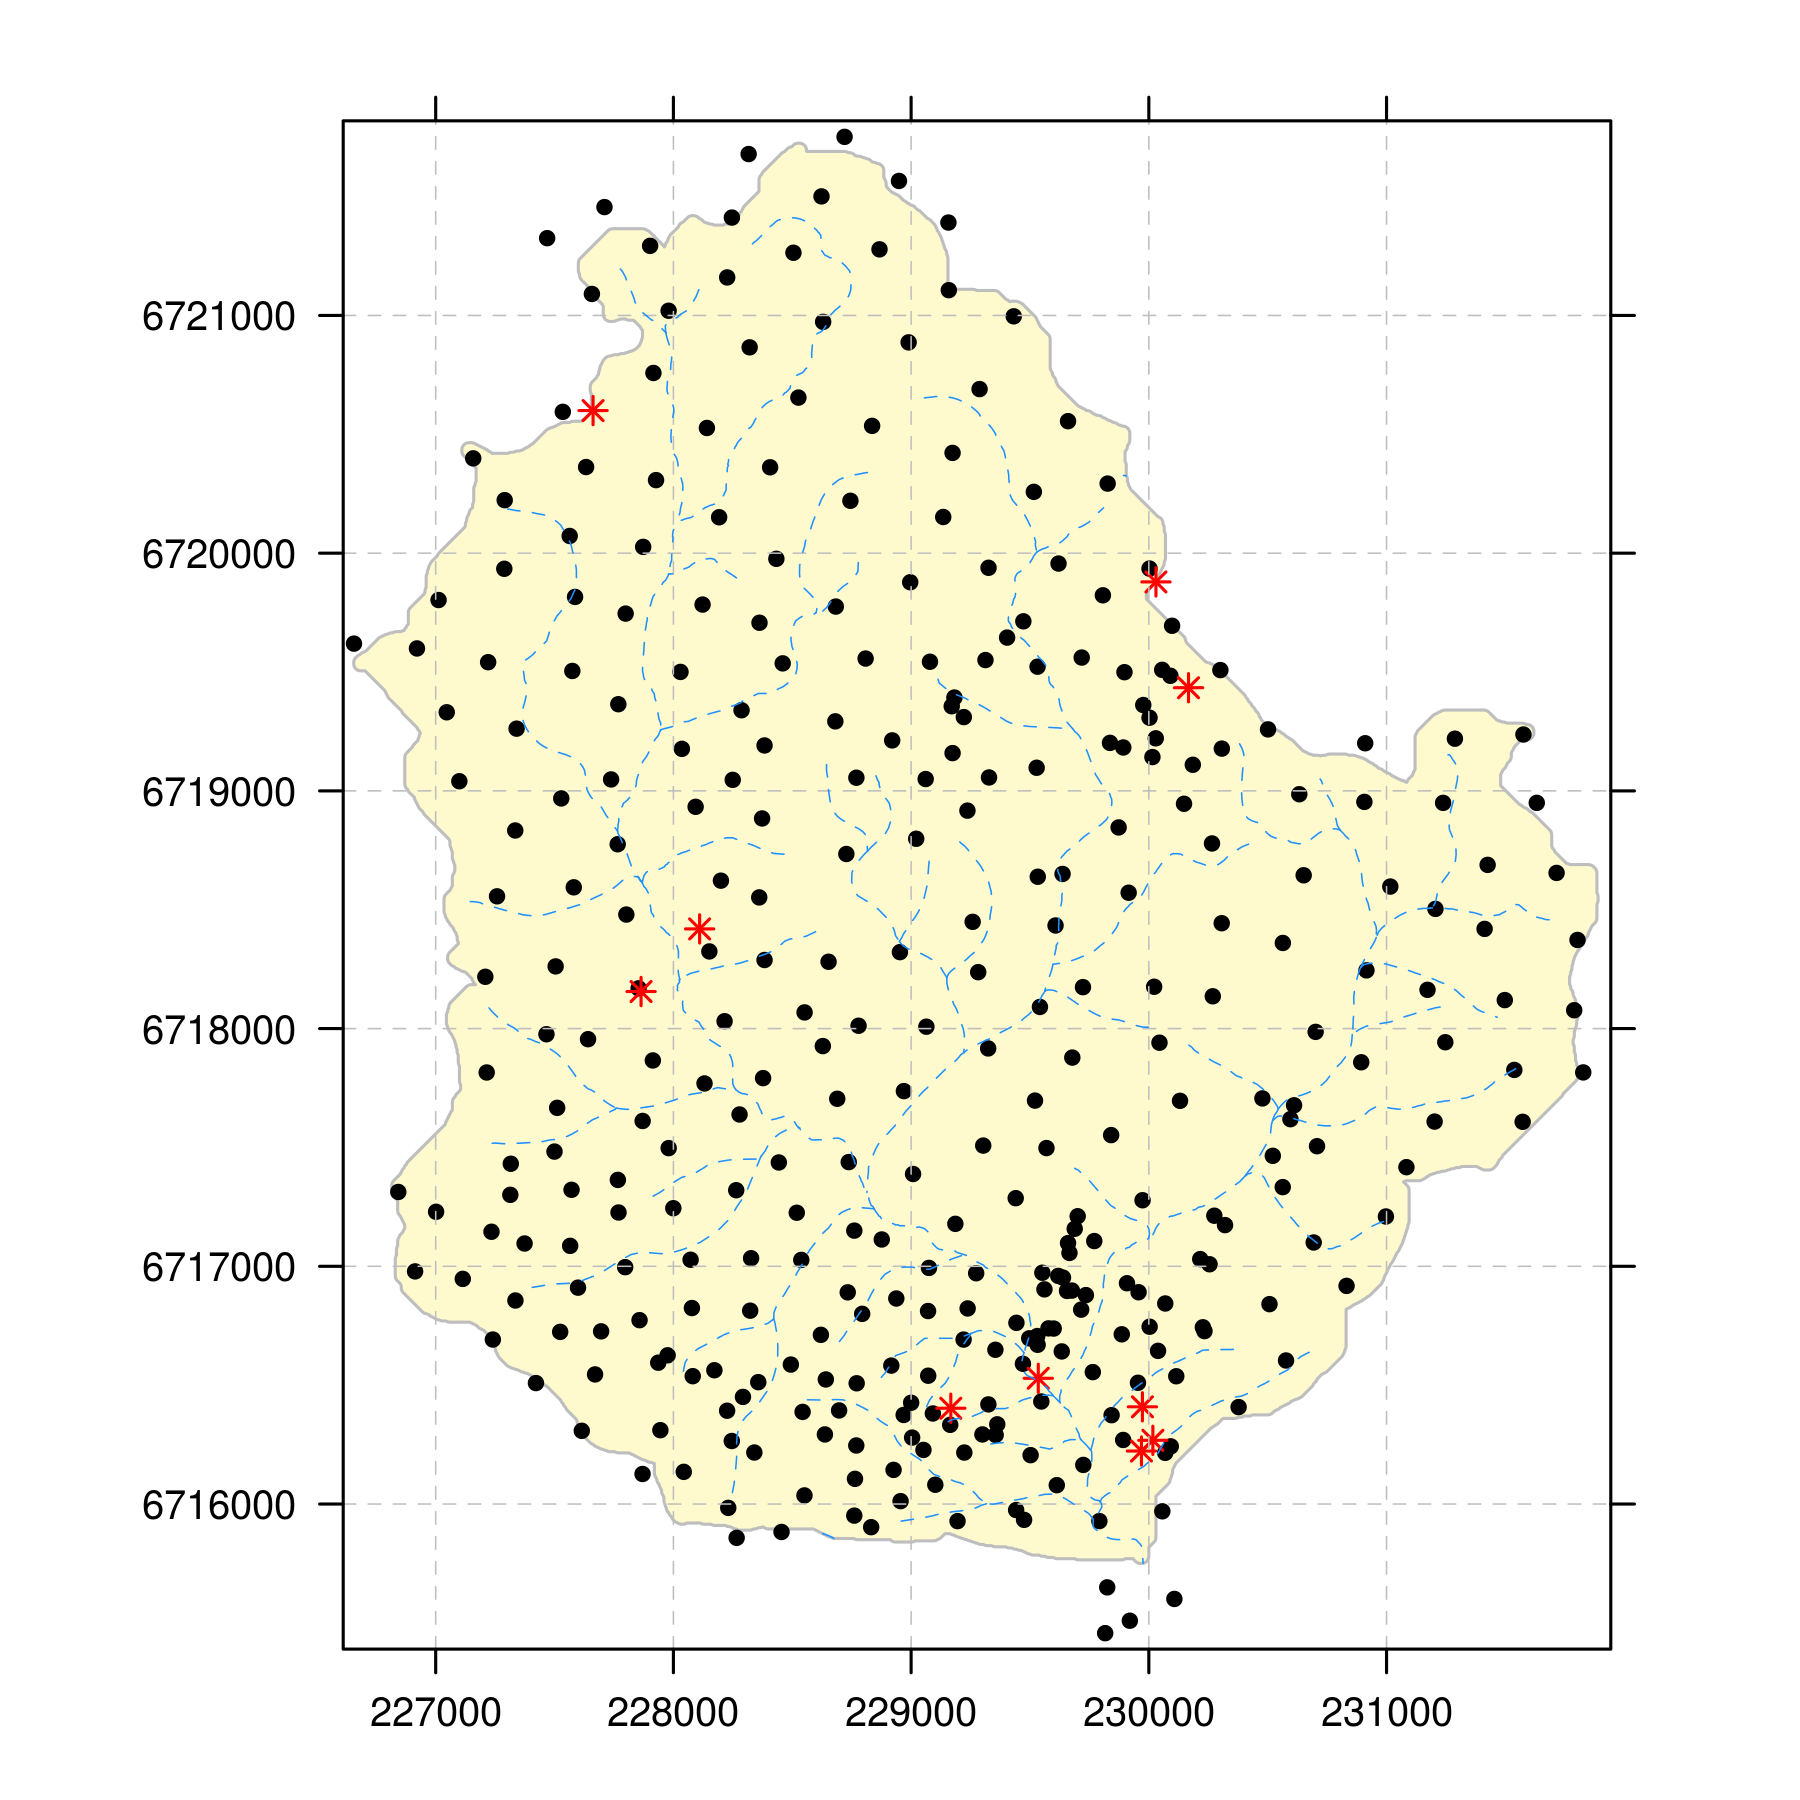
\includegraphics[width=0.90\textwidth]{fig/chap04-subsets-I-III}
\caption[Spatial distribution of \emph{Subset I} and \emph{Subset III}.]{Spatial distribution of the point soil 
observations contained in \emph{Subset I} ($n = 340$, black) and \emph{Subset III} ($n = 10$, red) of the Santa 
Maria dataset. The drainage network is shown in the background to give an idea of how the locations of soil 
observations is related to terrain features.}
\label{fig:chap04-subsets-I-III}
\end{figure}

Georeferencing was done in the field using a Global Navigation Satellite System (GNSS) receiver with a 
horizontal positional error of less than \SI{\pm8}{\metre} positioned approximately at the centre of the
sampling area. Sometimes, the horizontal positional error was larger than \SI{\pm8}{\metre} due the effects
of vegetation, terrain, and satellite configuration. In these cases, observation locations 
were georeferenced in the office using \SI{1}{\metre} spatial resolution \googleearth{} imagery with 
positional 
horizontal error of \SI{\pm6}{\metre} (\autoref{tab:chap05-google-geo-val}).

Every observation was identified with a number in increasing order, following the order in which the 
observations were made (\num{001}--\num{340}). A total of \num{17}~field campaigns were carried out, yielding 
an observation density of about \num{18}~observations per \si{\kilo\metre\squared}.

\subsection{Subset II}
\label{sec:chap04-subset-ii}

The second subset ($n = 60$) was produced in the years \num{2012} and \num{2013}, and was intended to 
constitute an independent dataset for validation purposes. Because of the many access limitations 
(geographic barriers and prohibition by landowners) and shortage of workforce, budget, infrastructure and 
time faced in previous field campaigns, researchers chose to employ transect (cluster) sampling 
\cite{MiguelEtAl2012, Moura-BuenoEtAl2012, Samuel-RosaEtAl2013}. They started defining the population of 
transects using their knowledge of the study area, taking into account the factors that they thought 
determined the spatial distribution of soil properties. Each researcher (three) delineated $m = 60$ easily 
accessible, straight transects of \SI{400}{\metre} following the spatial gradients of selected environmental 
features 
(topography, geology, vegetation, land use, and soils), totaling 180 transects. Accordingly, knowledge of 
existing roads, human 
settlements, water bodies, and other access limitations was used as well. The activity was carried out using 
\googlearth{} imagery of the years of \num{2008} and \num{2009}.

% TODO: add a figure with all transects highlighting the selected ones.
% \caption{Three experts drawn 180 linear transects aligned in the direction of maximum expected 
% spatial variance of environmental features. They avoided locations where it was known that geographic 
% barriers or landowners would impede the access to collect soil samples. Using probability sampling, 12 
% transects were selected to collect validation observations (red).}

Twelve out of the $m = 180$ transects were randomly selected using as many iterations as necessary until 
there were no intersecting transects, and there was at least one transect in each of the three major 
geomorphological units of the study area (\textit{Planalto}, \textit{Rebordo do Planalto}, and 
\textit{Depressão Periférica}). 
Finally, $n = 5$ observation locations, separated by equidistant intervals of \SI{100}{\metre}, were 
selected in each transect. Observation locations were named with a number in increasing order, 
following the order in which the observations were made, starting from \num{341} (\num{341}--\num{400}).

Observation locations were identified in the field using a GNSS receiver with a horizontal positional error
of less than \SI{\pm8}{\metre}. A single soil pit was opened within a radius of \SI{2}{\metre} from the 
predefined 
observation location. Soil sampling and description was carried out using the same procedure used with 
\emph{Subset I}, except that in Subset II a single pit was observed. More accurate geographic coordinates were 
collected in the field using a Differential Global Positioning System (DGPS) with a horizontal positional error 
of less than \SI{1}{\centi\metre}.

\subsection{Subset III}

The third subset ($n = 10$) contains data compiled from the studies of \citeonline{Pedron2005} and
\citeonline{Miguel2010}, specifically from the uppermost A horizon of modal soil profiles whose locations 
were purposively selected using tacit knowledge after a preliminary area-class soil map had been produced 
and/or the observations included in \emph{Subset I} had been made. The researchers aimed at observation 
locations that they understood as being most representative of the soil mapping units depicted in their 
respective area-class soil maps. A single soil sample was taken from each of the described soil horizons and 
used for laboratory analysis (see below). The resulting depth of the uppermost A horizons varies from \num{12} 
to \SI{30}{\centi\metre}, with a mean of \SI{22.6}{\centi\metre}. Georeferencing was carried using a GNSS 
receiver with a horizontal positional error of less than \SI{\pm8}{\metre} positioned at the observation 
location. Data are identified in the Santa Maria dataset using the same identification that was used in the 
studies from where they were compiled.

\section{FIELD DESCRIPTION}

Several environmental features were described at the observation locations. The next sections present a 
description of how this was done.

\subsection{Land Use}

Land use (\texttt{LAND}) was assessed in the years of \num{2008} and \num{2009} using data collected in the 
field and Google Earth imagery. Five land uses were identified: native forest (primary or secondary), 
shrubland 
(abandoned areas with predominance of shrub-sized vegetation, known in Brazil as \emph{capoeira}), animal 
husbandry (grasslands), forestry (\textit{Eucalyptus spp.} and \textit{Pinus spp.}), and annual crop 
agriculture. Other 
land uses such as human settlements and water bodies were not observed/sampled.

\subsection{Geology}

Soil parent material (\texttt{PARENT}, sedimentary or igneous), geologic formation (\texttt{GEO}), and 
lithology (\texttt{LITHO}) was inferred from direct observation of soil properties and local environmental 
features in the field. Existing geologic maps were used only when soil characteristics and environmental 
features were insufficient to reach an agreement about the most likely soil parent material, geologic 
formation, and lithology.

\subsection{Soil Classification}

The most likely soil classification (\texttt{TAXON}) was inferred in the field using direct observation of 
soil 
properties (\SI{20}{\centi\metre}-deep soil pits and auger holes down to the diagnostic subsurface horizon or 
bedrock) and local environmental features. Soil taxon was inferred only to the second categorical level of 
the Brazilian System of Soil Classification \cite{SantosEtAl2013a} because further levels require data that 
were not observed in the field.

% TODO: move this description of the soil taxa to the metadata file.
% RF - Neossolo Flúvico, RL - Neossolo Litólico, RR - Neossolo Regolítico, RQ - Neossolo 
% Quartzarênico, PV - Argissolo Vermelho, PVA - Argissolo Vermelho-Amarelo, PA - Argissolo 
% Amarelo, PBAC - Argissolo Bruno-Acinzentado, SX - Planossolo Háplico, CX - Cambissolo Háplico.

\subsection{Slope}

The slope gradient (\texttt{SLOPE}, \si{\percent}) was measured using a clinometer, the observer and target 
being at a constant height above the ground. The distance between observer and target was between 
\SI{30}{\metre} (dense forests) and \SI{50}{\metre} (open fields).

\subsection{Drainage}

Soil drainage status (\texttt{DRAIN}) was inferred visually from soil features observed with an auger using 
the 
classification scheme proposed by \citeonline{SantosEtAl2013}.

\subsection{Coarse Fragments and Rock Outcrops}

Presence of coarse fragments (\texttt{FRAG}) -- soil material of diameter \SI{>2}{\milli\metre} -- was 
described as a binary variable, that is, a value of \num{1} (one) was annotated when coarse fragments were 
present, and \num{0} (zero) otherwise. The same approach was adopted to describe the presence of rock outcrops 
(\texttt{ROCK}). The quantity of coarse fragments (\texttt{GRAVEL}, \si{\percent}) was estimated visually in 
some observation points.

It is worth noting that the approach employed to describe the presence of coarse fragments and rock outcrops is 
not in line with the standard soil description guidelines currently used in Brazil. The reason for this is that 
these soil properties were understood as being secondary at the time of sampling. As such, it seemed reasonable 
to record only their presence/absence.

\subsection{Canopy}

% TODO: add three figures as examples of each class.
Soil coverage with vegetation (\texttt{CANOPY}) was inferred visually in the field using three classes: low 
(\SI{<25}{\percent}), medium (\SIrange{25}{75}{\percent}), and high (\SI{>75}{\percent}).

\subsection{Additional Information}

Additional information was recorded at each observation location during the field campaigns. They refer to 
peculiarities of each observation location and were not recorded in a systematic way.

\section{LABORATORY ANALYSIS}
\label{sec:chap04-laboratory}

Soil samples were air dried, crushed and passed through a \SI{2}{\milli\metre}-sieve prior to laboratory 
analyses using the methods described in the next sections. One or more laboratory replicates were used to 
calculate analytical errors.

\subsection{Soil Organic Fraction}
\label{sec:chap04-organic}

The soil organic carbon content (\texttt{ORCA}, \si{\gram\per\kilo\gram}) was determined using the method of
\citeonline{Mebius1960} modified by \citeonline{YeomansEtAl1988} as described by \citeonline{ClaessenEtAl1997}.

\def\footsulfochromic{\footnote{See a detailed description of the sulfochromic solution, or chromic acid, at 
\href{http://en.wikipedia.org/wiki/Chromic_acid}{Wikipedia}.}}

Sample aliquots of \num{0.050} to \SI{0.500}{\gram} were placed in glass digestion tubes 
(\SI{80}{\milli\liter}). The amount of sample used varied according to the ORCA estimated by visual 
interpretation of soil colour. Every digestion tube received an aliquot of \SI{10}{\milli\liter} of 
sulfochromic solution\footsulfochromic{} [\SI{0.067}{\mole\per\liter} potassium bichromate solution
(\ce{K2Cr2O7}) in the presence of concentrated sulphuric acid (\ce{H2SO4})] and a small reflux funnel 
to avoid loss of reagent during digestion. A digestion block with capacity for \num{40}~samples was used:
\num{36}~tubes with soil sample plus \num{3}~tubes with blank plus \num{1}~tube with \ce{H2SO4} and a
thermometer for temperature control. Digestion at \SI{150}{\celsius} last \SI{30}{\minute}. Three blanks 
were prepared and set aside at room temperature to estimate the loss of reagent due to heat in the digestion 
block. After digestion the tubes were set aside at room temperature to cool down. Next, the solution was 
transferred to Erlenmeyer flasks (\SI{250}{\milli\liter}) with \SI{60}{\milli\liter} of distilled water and
\SI{2}{\milli\liter} of concentrated orthophosphoric acid [\ce{H3PO4}] and \num{3}~drops of 
\SI{1}{\percent}~diphenylamine). The solution was titrated using \SI{0.1}{\mole\per\liter} ammonium ferrous
sulphate (\ce{FeSO4(NH4)2 * 6H2O}) until persistent green colour. The results were multiplied by \num{1.11}
to correct to the standard method (dry combustion).

The soil organic matter content of the observations compiled from \citeonline{Pedron2005} was determined 
using the method described by \citeonline{TedescoEtAl1995}. Sample aliquots of \SI{2.5}{\milli\liter}
were placed in Erlenmeyer flasks (\SI{50}{\milli\liter}). Every Erlenmeyer flask received an aliquot of 
\SI{15}{\milli\liter} of \SI{0.067}{\mole\per\liter} sulfochromic solution (\ce{Na2Cr2O7 + H2SO4}). The 
flasks were heated in a water bath at \num{75} to \SI{80}{\celsius} during \SI{30}{\minute} and shaken 
for \SI{5}{\minute}. A water aliquot of \SI{15}{\milli\liter} was added to the flask and let overnight 
(\num{15} to \SI{18}{\hour}). In the next day, an aliquot of \SI{3.0}{\milli\liter} was sampled to a 
small cup with \SI{3.0}{\milli\liter} of distilled water. The absorbency of the supernatant was measured 
at \SI{645}{\nano\metre}. The results were transformed to organic carbon content using the Van Bemmelen 
factor (\num{1.724}), the result assumed to be equivalent to soil organic carbon content measured using the 
standard method. The results are expressed using a volume-basis and were converted to a mass-basis using a
1:1 relation because the mass of the sample aliquot used in the analyses is unknown.

\subsection{Particle Size Analysis}
\label{chap:chap04-granulometry}

\def\footsuzuki{\footnote{As far as I know, a comprehensive description of this method has not been 
published so far, neither in Portuguese nor in English. You can visit the homepage of the Soil Physics 
Laboratory of the Universidate Federal de Santa Maria at \url{https://coral.ufsm.br/fisicadosolo/} to get more 
information about the method or contact their developers.}}

Particle size analysis was performed using the pipette method, with the sand fraction (\texttt{SAND}, 
\SIrange{0.053}{2}{\milli\metre}, \si{\gram\per\kilo\gram}) determined by wet sieving, and the silt fraction 
(\texttt{SILT}, \SIrange{0.002}{0.053}{\milli\metre}, \si{\gram\per\kilo\gram}) calculated by difference. 
The analytical procedure is an adaptation\footsuzuki{} of the method of the Soil Conservation Service of 
the United States Department of Agriculture \cite{UnitedStates1972} made by the Soil Physics Laboratory of the 
\textit{Universidade Federal de Santa Maria} \cite{SuzukiEtAl2004, SuzukiEtAl2004a}.

First, a sample aliquot of \SI{20}{\gram} was placed in a \SI{100}{\milli\liter} glass container (height: 
\SI{10.5}{\centi\metre}; diameter: \SI{2.75}{\centi\metre}; weight: \SI{85}{\gram}). Two nylon spheres with a 
diameter of \SI{1.71}{\centi\metre} and weighting \SI{3.04}{\gram} (density: \SI{1.11}{\g\per\cm\cubic}) were 
added to act as physical disaggregating agents. Then, an aliquot of \SI{10}{\milli\liter} of 
\SI{1}{\mole\per\liter} sodium hydroxide (\ce{NaOH}) solution was added to act as chemical dispersing agent 
along with \SI{40}{\milli\liter} of distilled water. The glass container was closed with a plastic cap, 
manually shaken for \SI{10}{\second}, and placed in a horizontal mechanical shaker with capacity for 
\num{85}~samples. The suspension was left to stand overnight (\SI{10}{\hour}). In the next day the suspension 
was submitted to horizontal mechanical agitation during \SI{4}{\hour} at \si{120} cycles per minute 
\cite{SuzukiEtAl2004, SuzukiEtAl2004a}.

After horizontal agitation, the suspension was poured in a plastic graduated cylinder with capacity for 
\SI{1000}{\milli\liter} using a glass funnel and a metal sieve to hold the two nylon spheres. The suspension 
in 
the graduated cylinder was completed to \SI{1000}{\milli\liter} and homogenized using a hand stirrer 
(\SI{30}{\second}). The suspension was allowed to stand until sedimentation was complete. The time needed was 
calculated using the Stokes’ law with the temperature measured in a graduated cylinder filled with distilled 
water.

%TODO provide a more detailed description of how CLAY was determined as well as of the oxidative
%treatment with H2O2.

The clay fraction (\texttt{CLAY}, \SI{<0.002}{\milli\metre}, \si{\gram\per\kilo\gram}) was determined by the 
pipette method. Soil samples with organic matter content \SI{>5}{\percent} were submitted to oxidative 
treatment with hydrogen peroxide (\ce{H2O2}) prior to the analysis following the recommendations of
\citeonline{ClaessenEtAl1997}.

%The sand fraction was separated into five size classes:
%
%\begin{itemize}
%\item \SIrange{1.00}{2.00}{\milli\metre}: very coarse sand;
%\item \SIrange{0.50}{1.00}{\milli\metre}: coarse sand;
%\item \SIrange{0.25}{0.50}{\milli\metre}: median sand;
%\item \SIrange{0.106}{0.25}{\milli\metre}:fine sand;
%\item \SIrange{0.053}{0.106}{\milli\metre}: very fine sand.
%\end{itemize}

% The clay fraction (\textless0.002~mm) was initially determined by the pipette method without any 
% pretreatment. A 1~mol~L$^{-1}$ NaOH solution was used as the dispersing agent, with the addition of two 
% nylon spheres as disaggregating agent plus horizontal mechanical agitation during 4~hours 
% \cite{SuzukiEtAl2004}.

% A propor{\c{c}}{\~{a}}o da fra{\c{c}}{\~{a}}o argila dispersa em {\'{a}}gua foi determinada conforme 
% descrito acima para a fra{\c{c}}{\~{a}}o argila total. A diferen{\c{c}}a {\'{e}} que n{\~{a}}o foi usado o 
% agente dispersante (NaOH) e o agente desagregante (esferas de nylon) \cite{ClaessenEtAl1997}.

\subsection{Soil Density}
\label{chap:chap04-bude}

% TODO: Provide a more detailed description of how this is done.
The bulk soil density (\texttt{BUDE}, \si{\mega\gram\per\cubic\metre}) was determined using the core method 
with a metallic ring (height: \SI{3}{\centi\metre}; diameter: \SI{5}{\centi\metre}) as described by 
\citeonline{ClaessenEtAl1997}. The bulk soil density was not determined in the locations where the soil was 
very shallow or stony.

\subsection{Exchangeable Bases and Acidity}
\label{chap:chap04-ecec}

The exchangeable calcium (\texttt{CALC}, \si{\milli\mole\per\kilo\gram}) and magnesium (\texttt{MAGN}, 
\si{\milli\mole\per\kilo\gram}) were determined by atomic absorption spectroscopy after extraction with 
\SI{1.0}{\mole\per\liter} \ce{KCl} solution using the method described by \citeonline{ClaessenEtAl1997}. 
The exchangeable sodium (\texttt{SODI}, \si{\milli\mole\per\kilo\gram}) and potassium (\texttt{POTA}, 
\si{\milli\mole\per\kilo\gram}) were extracted with a \SI{0.05}{\mole\per\liter} \ce{HCl} solution plus 
\SI{0.025}{\mole\per\liter} \ce{H2SO} (Mehlich-\num{1} solution). Both were quantified by means of flame 
atomic emission spectrometry using the method described by \citeonline{TedescoEtAl1995}.

The exchangeable acidity (\texttt{EXAC}, \si{\milli\mole\per\kilo\gram}) was extracted using the same 
\SI{1.0}{\mole\per\liter} \ce{KCl} solution used to extract the exchangeable calcium and magnesium. It was 
determined by titrimetry with \SI{0.025}{\mole\per\liter} \ce{NaOH} solution as described by 
\citeonline[p.~103]{ClaessenEtAl1997}.

% TODO: Include POAC in the database and improve the description of how it was determined.
% The potential acidity (POAC, \si{\milli\mole\per\kilo\gram}) was determined with \SI{1.0}{\mole\per\liter} 
% calcium acetate solution at pH~\num{7.0} and titrated with \SI{0.0606}{\mole\per\liter} \ce{NaOH} solution 
% as described by \citeonline{ClaessenEtAl1997}.

The effective cation exchange capacity (ECEC, \si{\milli\mole\per\kilo\gram}) was defined as the sum of 
exchangeable bases and exchangeable acidity, i.e. 

\begin{equation*}
 \texttt{ECEC} = \texttt{CALC} + \texttt{MAGN} + \texttt{POTA} + \texttt{SODI} + \texttt{EXAC}.
\end{equation*}


% TODO: Provide a more detailed description of how these are calculated and include the data in the database.
% The sum of exchangeable bases (BASES) is given by the sum of the exchangeable calcium, magnesium, sodium and 
% potassium. The effective cation exchange capacity (ECEC) is given by the exchangeable acidity plus the 
% sum of exchangeable bases. The potential cation exchange capacity (CEC) is given by the potential acidity 
% plus the sum of exchangeable bases. Note that the standard method for determining exchangeable bases relies 
% on the use of barium chloride [BaCl$_2$]. The base saturation (BASA) is given by the sum of exchangeable 
% bases divided by the potential cation exchange capacity. The saturation of the ECEC with exchangeable 
% acidity, or the aluminum saturation (ALSA), is given by the sum of exchangeable bases divided by the 
% effective cation exchange capacity. The results are multiplied by 100. 

% \begin{figure}[!ht]
% \centering
% <<echo = FALSE>>=
% options(useFancyQuotes = FALSE)
% tmp <- read.table(
%  '~/projects/dnos-sm-rs/dnos-sm-rs-general/data/labData.csv', sep = ";",
%  header = TRUE, na.strings = 'na')
% lattice::trellis.par.set(
%  fontsize = list(text = 16, points = 15), axis.line = list(lwd = 0.01),
%  layout.widths = list(left.padding = 0, right.padding = 0),
%  layout.heights = list(top.padding = 0, bottom.padding = 0))
% aa <- pedometrics::plotHD(tmp$CLAY, xlab = 'CLAY')
% bb <- pedometrics::plotHD(tmp$ORCA, xlab = 'ORCA')
% cc <- pedometrics::plotHD(tmp$ECEC, xlab = 'ECEC')
% dd <- pedometrics::plotHD(na.exclude(tmp$BUDE), xlab = "BUDE")
% @
% \begin{minipage}[b]{63mm}
% \subcaption{}
% \centering
% <<intro-clay, fig = TRUE, echo = FALSE>>=
% print(aa)
% @
% \end{minipage}
% \begin{minipage}[b]{63mm}
% \subcaption{}
% \centering
% <<intro-orca, fig = TRUE, echo = FALSE>>=
% print(bb)
% @
% \end{minipage}
% \begin{minipage}[b]{63mm}
% \subcaption{}
% \centering
% <<intro-ecec, fig = TRUE, echo = FALSE>>=
% print(cc)
% @
% \end{minipage}
% \begin{minipage}[b]{63mm}
% \subcaption{}
% \centering
% <<intro-bude, fig = TRUE, echo = FALSE>>=
% print(dd)
% @
% \end{minipage}
% \caption{The four soil properties explored in this thesis: (a) clay content, (b) organic carbon
% content, (c) effective cation exchange capacity, and (d) bulk density. Each panel shows the sample
% histogram and summary statistics of the soil properties in their original scale ($\lambda = 1$), as
% well as the theoretical probability density function so that we can assess how good is the fit of
% the normal distribution to the data -- a product of the \Rpackage{pedometrics}.}
% \label{fig:intro-soil-properties}
% \end{figure}

\section{FINAL CONSIDERATIONS}

The main goal of documenting the soil data contained in the Santa Maria dataset was to provide the reader the 
basis to understand the soil data used in the thesis, and also to support future soil spatial modelling 
exercises in 
the catchment of the DNOS reservoir.

As a result of an ongoing collaborative effort, this documentation will be improved in the near future as new 
studies are developed. We plan to include new figures to exemplify how field soil sampling was carried out. 
Details of non-standard soil description and analysis methods will likely be extended. This includes the 
oxidative 
treatment with \ce{H2O2} to which soil samples were submitted prior to particle size distribution analysis. 
For 
cases such as the ECEC, determined using a non-standard method, we plan to develop a study to calibrate a 
model 
to convert our results to the standard method for determining exchangeable bases, which uses barium chloride 
(\ce{BaCl2}) for saturation.

Other already existing soil data will also be included in the Santa Maria dataset and documented as well. 
These 
data have not been used in any study so far, including the potential acidity, sum of exchangeable bases, 
potential 
cation exchange capacity, base saturation, aluminium saturation, and the five size classes of the sand 
fraction.

Once a comprehensive documentation of the existing soil data has been constructed, we will prepare a basic 
spatial exploratory soil data analysis. We hope that our effort to properly document the soil data that we 
produced,
and make it freely available for use, will serve as an example for future soil spatial modelling studies 
developed 
elsewhere.

